%% === Auto-generated by scripts/write_param_sweeps_snippet.py from results/param_sweeps.csv ===
%% Integration instructions:
%%  1. Insert the \begin{figure}...\end{figure} block below into Section 5 (Evaluation),
%%     immediately before \subsection{Sensitivity and Runtime} (sec:sensitivity).
%%  2. Replace the opening paragraph of that subsection (the one starting "DeclareCascade uses a
%%     single fixed configuration...") with the REPLACEMENT PARAGRAPH below.
%%  3. In the existing \begin{table*}...\end{table*} float (label tab:traceability /
%%     tab:xi-sweep), delete the second \begin{minipage}...\end{minipage} (tab:xi-sweep) and
%%     the \hfill before it, per the TABLE SURGERY note below -- tab:traceability then stands
%%     alone in the float.

%% ---------------------------------------------------------------------------
%% 1. New figure
%% ---------------------------------------------------------------------------
\begin{figure}[t]
\centering
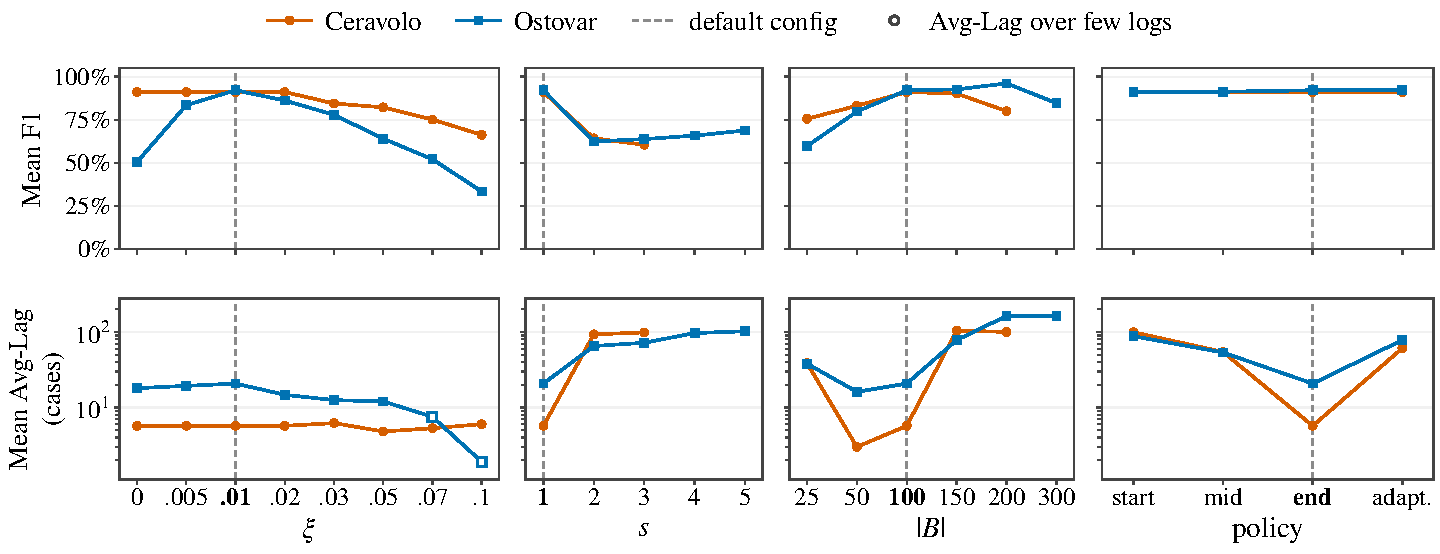
\includegraphics[width=\textwidth]{figures/fig5_param_sweeps.pdf}
\caption{Mean F1 (top) and mean localisation error (bottom, Avg-Lag in cases) across four
one-at-a-time sweeps of the detection configuration: the intensity threshold $\xi$, the
trailing-window width $s$, the batch size $|B|$, and the localisation policy. All other
parameters are held at the default (dashed guide, bold tick). $x$ axes are ordinal -- swept
values are equally spaced, so segment slope is not a derivative. A line is cut where fewer than
four boundaries remain statistically testable (ceravolo at s$\geq$4; ceravolo at B$\geq$300),
since an F1 computed over that few candidate boundaries is not meaningful; a hollow lag marker
denotes a mean Avg-Lag computed over fewer than 60\% of logs, since \texttt{get\_avg\_lag}
only averages logs with at least one true positive and a config that stops detecting reports the
lag of the few logs it still hits.}
\label{fig:param-sweeps}
\end{figure}

%% ---------------------------------------------------------------------------
%% 2. Replacement opening paragraph for Section 5.3 (Sensitivity and Runtime)
%% ---------------------------------------------------------------------------
DeclareCascade uses a single fixed configuration ($\vartheta\!=\!0.999$, $\xi\!=\!0.01$,
$s\!=\!1$, $|B|\!=\!100$, report$\,=\,$end) across both datasets without per-dataset tuning.
Figure~\ref{fig:param-sweeps} extends the sensitivity analysis from $\xi$ to the other three
detection parameters, sweeping each while holding the rest at that default.
%
The intensity threshold $\xi$ has a clear optimum at the chosen value: F1 is stable within
$\xi\in[0.005,\,0.02]$ and falls away on both sides, as noise dominates at lower thresholds
(Ostovar 0.505 at $\xi\!=\!0$) and recall collapses at higher ones
(0.333 at $\xi\!=\!0.10$, over only
27 of
75 logs).
%
The trailing window admits no such latitude: $s\!=\!1$ is strictly best, and widening it to
$s\!=\!2$ costs accuracy immediately (Ceravolo 0.911$\rightarrow$0.642,
Ostovar 0.922$\rightarrow$0.624) while inflating localisation error roughly
an order of magnitude (5.7$\rightarrow$92.9 and
20.7$\rightarrow$65.1 cases). A wider trailing window both re-tests
inside the same transition, re-firing on a drift it has already reported, and -- on a
1\,000-case log -- leaves too few boundaries statistically testable to judge at all.
%
The batch size $|B|$ exposes the granularity/power trade-off directly. Shrinking it does
\emph{not} buy better localisation as one might expect: at $|B|\!=\!25$ both F1 and lag
degrade (Ceravolo 0.756 at 38.6 cases, versus 0.911 at
5.7 at the default), because 25-case batches make the per-batch proportions too
noisy and the detector fires early and spuriously. Growing it past the default costs lag
outright, the reported change point being quantised to a coarser batch edge. The lag optimum sits
at $|B|\!=\!50$ (Ceravolo) and
$|B|\!=\!50$ (Ostovar), close to the default.
%
The five localisation policies, finally, separate cleanly from the other three parameters: F1 is
essentially flat across all of them (Ceravolo 0.911 for \emph{start} vs
0.911 for \emph{end}) while mean lag varies by more than an order of
magnitude, from 13.2 cases (\emph{end}) to
93.4 (\emph{start}, averaged over both datasets). This is
exactly what Section~\ref{sec:confirmation} claims structurally: the policy is applied after
confirmation and changes only \emph{where} inside the firing batch a detected change is
reported, never \emph{which} batches fire.

%% ---------------------------------------------------------------------------
%% 3. TABLE SURGERY (existing table* float, currently tab:traceability + tab:xi-sweep)
%% ---------------------------------------------------------------------------
%% DELETE this second minipage (and the preceding \hfill) from the existing \begin{table*}:
%%
%%   \hfill
%%   \begin{minipage}[c]{0.4\textwidth}
%%   ...
%%   \label{tab:xi-sweep}
%%   \end{minipage}
%%
%% tab:traceability then stands alone; widen its minipage from 0.58\textwidth to, e.g.,
%% 0.9\textwidth (or drop the minipage wrapper entirely and let the tabularx span the table*).
